\chapter{Related Work} % (fold) ===============================================
\label{cha:background}
Robotic systems capable of locomotion have existed for decades, with some of the earliest designs dating back to the late nineteenth century. Using a series of mechanical drivetrain components, Rygg developed a mechanical horse capable of generating fixed gait in 1893 \cite{rygg1893mechanical}. Several years later in 1988, Fallis developed the first \emph{passive} bipedal walking toy capable of stable gait \cite{pallis1888fallis}. The term \emph{passive} denotes the lack of any active power input to the system. Fallis's toy produced \emph{statically} stable walking, whereby the center-of-mass (COM) always remains within the base of support throughout the gait cycle. In contrast, the COM leaves the base of support during \emph{dynamically} stable gait. 

McGeer's seminal research \cite{McGeer:1990uk} nearly a century later produced \emph{passive} bipeds capable of dynamically stable gait without any control effort. This work led to a new class of passivity-based designs for bipedal robots. Similarly, pivotal research by Vukobratovic \cite{vukobratovic1969} introduced a dynamic measure of balance widely used in walking control strategies today. This sparked the rapid growth of actively-powered bipedal robot designs. The electromechanical design and gait synthesis method used to achieve bipedal locomotion are profoundly related. Bipedal robots are often designed to target a specific control strategy. This chapter presents a literature review of the related work in this research area. 


%==============================================================================
%   E L E C T R O M E C H A N I C A L   D E S I G N 
%==============================================================================



\section{Humanoid Electromechanical Design} % (fold) ==========================
\label{sec:related_electromechanical_design}
The first \emph{active} bipedal robot, WL-5 was developed in the 1972 by Kato et al. at Waseda University \cite{kato1972hydraulically}. Since then, the number of bipedal robots being developed for commercial and research applications has been growing rapidly. The main electromechanical design considerations for humanoid robots are reviewed in this section. 


\subsection{Degrees of Freedom} % (fold) ======================================
\label{sub:related_degrees_of_freedom}
A bipedal robot achieves locomotion by articulating the limbs connected by joints in the lower body. Therefore, the degrees-of-freedom (DOF) in the lower body of a humanoid robot plays an important role in bipedal locomotion. The obvious design parallel to draw inspiration for bipedal locomotion is from humans. However, the lower body of a human is difficult to model due to the large number of DOF formed by muscles and tendons. Therefore, the selection of lower body DOF is typically chosen to provide sufficient maneuverability while reducing redundant DOFs to the essential set required to achieve walking. 

The primary DOF used to articulate the lower body limbs are the hip, knee and ankle joints. A simpler design widely used in robotics literature is the 2-dimensional (2D) planar biped. This approach typically uses a 1 DOF hip and 1 DOF knee joint in conjunction with point feet \cite{tzafestas1996robust}. Physical implementations of these planar bipeds constrain its motion to the sagittal plane by using a boom \cite{chevallereau2000design,pratt2001virtual,Wight:2008vt}. 

The most common examples of \emph{active} 3-dimensional (3D) lower body designs use 3 DOF for the hip joint, 1 DOF at the knee and 2/3 DOF for the ankle joint \cite{Hirai1998,IllWooPark:2005et,Kaneko:2004wq,Ogura:2006bm,yamaguchi1999}. The hip joint is arguably the most complex joint to design as it must provide a wide range of motion and be capable of carrying the weight of each leg. Several bipedal robots use innovative hip joint designs to improve mobility and/or reduce the DOF. Aldebaraan's Nao robot strategically places the hip motors to reduce 1 DOF while maintaining a similar range of motion \cite{Gouaillier:2008ug}. The bipedal robot from the Japanese government's Humanoid Robot Project, HRP-2 utilizes a unique cantilever hip structure to enable cross-legged walking (i.e. on a tight rope) \cite{Kaneko:2004wq}. 

More recent research has been aimed at mimicing the large number of DOF present in humans through complex electromechanical designs. Musculoskeletal robots \cite{Mizuuchi:2007em,Osada:2010cj} generate a high (variable) number of DOF using complex actuation mechanisms to emulate muscles. The additional complexitiy and large DOF drastically increases the complexity of the control strategy. 

% subsection degrees_of_freedom (end) =========================================


\subsection{Mechanism Design} % (fold) ========================================
\label{sub:related_mechanism_design}
The mechanical design of linkages used in robotics largely fall into two categories, serial and parallel link manipulators. Serial link manipulators contain a series of joint-driven links that extend from the base to an end-effector. Parallel link manipulators on the other hand contain several (serial) links connecting a base to its end-effector. A well-known parallel link manipulator used in robotics is the 6 DOF Stewart-Gough platform \cite{Dasgupta2000,Sugahara2005}. The same parallel design technique can be scaled down to design high performance multi-DOF joints \cite{Gosselin1994}. A common application of this design approach in the lower body of a humanoid is for spherical joints (i.e. 3 DOF) hip joint \cite{Hofschulte2005}. 

The primary motivation for investigating serial vs. parallel mechanism design for lower body humanoid robots is to improve the performance of the system. The majority of the mass of a robot joint-link assembly comes from the actuator. It is often useful to manipulate the overall weight distribution to improve the system behaviour under control action. For example, a common approach used in bipedal locomotion is to approximate the dynamics during single support phase as an  inverted pendulum \cite{Kajita1992}. In this approach, the swinging leg is assumed to be massless. Having larger motors further down along the swing leg introduces a larger inertia and consequently influences the stability during walking \cite{Morisawa2000}. Therefore, it is common to manipulate the weight distribution in the lower body to raise the COM and improve the system performance. 

Serial link manipulators have the benefit of straight forward design and kinematics, making it easier identify singular configurations in the joint space. However, these mechanisms suffer from poor accuracy since position error accumulates at each link of the chain and poor dynamic performance since the inertial effect of each link can not be neglected \cite{Merlet2006}. Despite these drawbacks, some of the most famous humanoid robots use serial mechanisms, including the Honda ASIMO \cite{Sakagami:2002cf} and Waseda University's WABIAN-2 \cite{Ogura:2006bm}. The serial arrangement of actuator-driven joints also make it difficult to relocate actuators from each joint axis for better weight distribution. Mechanical transmission components (i.e. belts, pulleys, gears) are often used to disconnect the actuator output from the joints \cite{Ogura:2006bm}. However, this also introduces additional complexity which is difficult to model (i.e. slop introduced by a belt-pulley system) and often requires tuning \cite{IllWooPark:2005et}. 

On the other hand, the parallel link manipulators enable easier relocation of actuators. Parallel joints also distributes the torque requirements equally across all actuators, which in turn reduce the individual actuator size and improves the power-to-weight ratio \cite{Lohmeier2006,Konno2002}. Due to these reasons, it was found that the energy consumption of parallel linked structures is significantly lower than that of its serially linked counter part \cite{Morisawa2000}. Parallel joints also provide the benefit of high stiffness and accuracy \cite{Sellaouti2005}. However, it is much more difficult to determine the singular configurations of the parallel structure without kinematic analysis \cite{Sellaouti2005}.

% subsection mechanism_design (end) ===========================================


\subsection{Passivity-Based Designs} % (fold) =================================
\label{sub:related_passive_designs}
The most simple bipedal robot designs are purely mechanical devices which are capable of walking without any active power. Inspired by the field of passive dynamics, these bipeds rely on the natural dynamics of the system for gait generation. McGeer first demonstrated this concept on a simple mechanical system consisting of two straight legs connected by a hinge at the hip \cite{McGeer:1990uk}. This initial design was revised by adding knees for more anthropomorphic gait and to solve the foot clearance issue during the recovery phase \cite{McGeer:1990hh}. Nearly a decade later, Garcia et al. performed an indepth analysis on the speed, efficiency and mechanism design of 2D passive dynamic walkers \cite{Garcia:2000kv}. Several design options were investigated for passive 2D bipeds, including kneed and straight-legged models with round and point feet. A four legged lower body design (inner and outter pairs) was adopted for physical implementations to constrain the problem to 2D and prevent falling sideways. Collins et al. built the first 3D passive bipedal robot which used swinging arms to counteract the sideways instability \cite{Collins:2001jq}. This passive design was capable of producing remarkably human-like gait without any active power input. 

The purely passive mechanical designs relied on gravitational power and sloped inclines. However, the passivity-based design techniques were extended to achieve walking on level ground by substituting gravitional power with minimal actuation \cite{Collins:2005vp}. This produced energetically efficient 3D bipedal robots based on passive dynamics principles. Delft University's bipedal robot Denise was designed with cylindrically shaped feet and a mechanical link to couple the forward motion of one leg to the reverse motion of the other \cite{Anderson:2005cw}. Minimal actuation is provided at the hip joint to achieve walking on level ground. Flame, the most recent energetically efficient 3D bipedal robot from Delft University, was designed specifically to take advantage of the natural dynamics of the system \cite{Hobbelen2008}. The electromechanical design was aimed towards obtaining high compliance and low control stiffness by using series elastic actuators (SEA). Other common actuation strategies used for passivity-based designs include pneumatics and hydraulics. 


Pneumatics is used to generate mechanical power through pressure manipulation within a membrane by an air compressor. The main advantage of this actuation strategy is its high power-to-weight ratio and inherent compliance \cite{Wisse2007}. Electromechanical designs based on this type of actuation use variations of Pneumatic Artificial Muscles (PAM) to control joint motion. The most common variation used in lower body joints is the McKibben muscle (braided PAM). Delft University has produced several robots Mike \cite{Wisse2003}, Max \cite{Hobbelen2005} and Denise \cite{Hobbelen2008,Wisse:2007wh} which use McKibben muscles for minimally actuated walking. VUB's planar biped Lucy based on pleated PAM actuators was used to explore energetically efficient walking with adaptable compliance \cite{Vanderborght:2005kq}. The major drawback of pneumatic actuators is its low position accuracy and non-linear response. 

Hydraulics is used to generate mechanical power through pressure manipulation of oil from a hydraulic pump. Flow control valves are used to regulate the hydraulic pressure in a hollow cylinder, which in turn manipulates a linear force applied through a piston. The linear force is applied to a moment arm producing a torque at the joint. The main advantage of this actuation strategy is its high power density and inherent compliance. The SARCOS humanoid CB is a force-controllable biped with hydraulic actuators \cite{SangHoHyon:2007jy}. The non-linear properties of hydraulic actuators make joint level control a challenging task. Impedance control schemes are used to reduce the non-linear effects and compensate for unmodeled dynamics \cite{Bilodeau1998}. In addition to the modeling complexities, the major drawbacks of using hydraulic actuators is that it is expensive and a pump is required supply the high pressure oil through hydraulic hoses to each joint. This increases the design complexity and introduces additional points of failure.

% subsection passivity_based_designs (end) ====================================


\subsection{Actively-Powered Designs} % (fold) ================================
\label{sub:related_active_designs}
The most common approach to electromechanical design for bipedal robots is through the generation of active power for locomotion. As opposed to the minimally actuated approach used in passivity-based designs, most actively-powered bipeds require a high degree of accuracy for controllability. Actuation strategies like SEA, pneumatics and hydraulics have non-linear behaviour which is difficult to model and control. In contrast, the strategy used for most complete actively-powered designs rely on electric machines. 

Electric machines are commonly used in humanoid robotic applications due to the high precision of control at the output shaft. Electromechanical designs based on this type of actuation use AC motors, DC motors or servomotors sized to handle a variety of loads. Some humanoid robots have custom built electric machines designed specifically to improve the performance for the intended application (i.e. the Honda humanoid robots \cite{Sakagami:2002cf,Hirai1998}). Electric machines drive the link motion through either direct or geared drive mechanisms. In direct drive, the motor shaft is mounted to drive the joint directly producing low torques and high speed. Geared drives are often used to increase the motor torques and lower the shaft speed through a gear reduction ratio.

Standard gearing mechanisms (i.e. planetary, spur gears) suffer from the backlash problem while other high end (expensive) options like harmonic drives do not. Waseda University's WABIAN-2 robot combines a DC motor with harmonic drive for every actuation system \cite{Ogura:2006bm}. Alternatively, KAIST's HUBO robot selectively uses harmonic drives only in the lower body since backlash in these joints can affect the overall stability of the system \cite{IllWooPark:2005et}. The major drawback of using electric machines is their high mechanical impedence (no compliance) and drivetrain losses when coupled with geared drive mechanisms.  
% subsection actively_powered_designs (end) ===================================


% section humanoid_electromechanical_design (end) =============================



%======================================================================
%   W A L K I N G  C O N T R O L  &  G A I T  G E N E R A T I O N
%======================================================================



\section{Walking Control Strategies and Gait Generation} % (fold) =============
\label{sec:related_control_strategies}
There exists a wide range of walking control strategies and gait generation methods to achieve bipedal locomotion. Some of the most popular strategies are briefly reviewed in this section.


\subsection{Zero-Moment Point} % (fold) =======================================
\label{sub:related_zero_moment_point}
The most popular techniques to achieve walking have been trajectory generation and control strategies based on the Zero-Moment Point (ZMP) criterion \cite{Vukobratovic:2004wy}. The ZMP defines a point on the ground where the forces acting on a biped do not produce a moment about the axes parallel to the ground plane (shown in Figure~\ref{fig:zmp}). The criterion states that the biped is stable if the ZMP is kept within the region of foot support at every time instant. The ZMP location is typically used as a feedback mechanism to achieve dynamically stable gait.  

\begin{figure}[!h]
	\begin{center}
    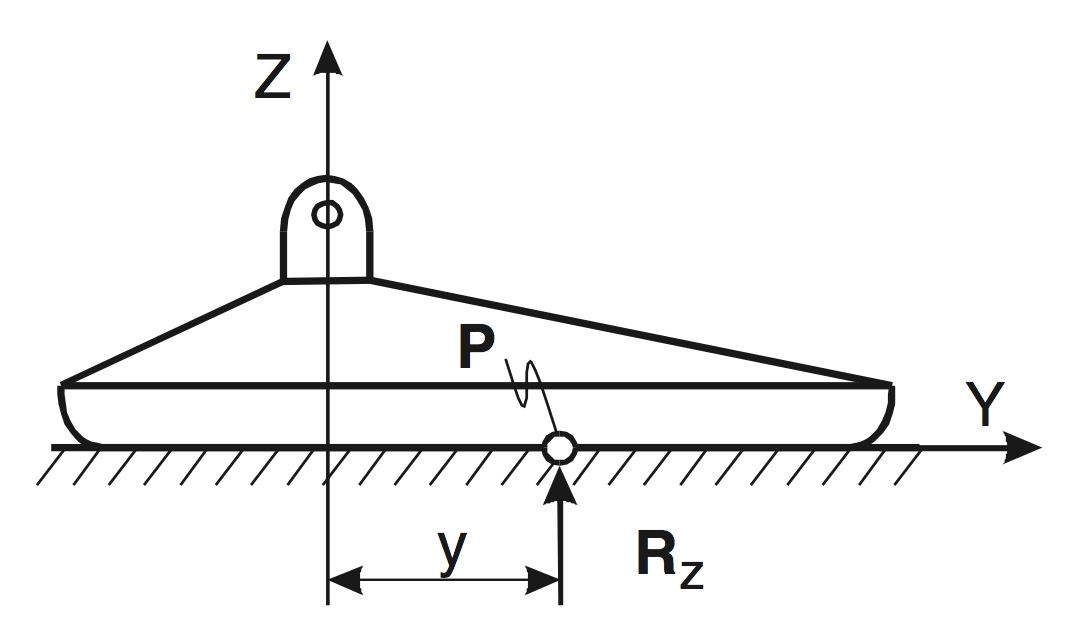
\includegraphics[scale=0.3]{fig/background/zmp.png}
	\end{center}
  \caption{Planar view of the ZMP location (indicated by point P) within the region of foot support.}
  \label{fig:zmp}
\end{figure}

This criterion can be used to pre-compute ZMP-stable trajectories offline. Huang et al. presented a walking pattern generation algorithm to compute the desired foot and hip trajectories offline \cite{HuangEtAlTRA2001}. This algorithm aimed to select a ZMP-stable hip trajectory which maximized the stability margin (distance from the ZMP point to the boundary of the support region). Computationally expensive exhaustive search was used offline to obtain the optimal solution for a given walking speed and step length. During the on-line phase, the selected optimal trajectories were tracked to execute walking.

Kajita et al. developed a walking pattern generation algorithm based on the 3D linear inverted pendulum mode (LIPM) \cite{Kajita:2001fk} and preview control \cite{KajitaEtAlICRA2003}. Using this approach, the desired swing foot positions can be adjusted on-line to compute a new ZMP trajectory which remains within the region of foot support. A ZMP tracking controller (based on the table-cart system) is used to generate the desired \emph{future} COM trajectory. The preview controller uses this future reference signal (within a specified time period) to generate the adjusted \emph{current} COM trajectory to remain dynamically stable. More recent methods use more accurate modeling techniques (instead of 3D LIPM) to compute ZMP-based trajectories on-line \cite{TakenakaEtAlIROS2009}. 

The biggest drawback of ZMP-based methods is the resulting trajectory does not provide any strategy to respond to disturbances due to uneven terrain or unexpected forces. Typically, these strategies are also energetically inefficient since they are constantly trying to maintain balance by keeping the ZMP point within the region of foot support. Furthermore, the resulting gait does not utilize the natural dynamics of the system and consequently does not look human-like.

Despite the drawbacks, some of the most popular humanoid robots for commercial and research applications utilize some variation of ZMP based feedback for bipedal locomotion. The well known Honda ASIMO \cite{Sakagami:2002cf} uses ZMP as part of its i-WALK technology (predicted movement control). Newer bipeds available for research like Aldebaraan's Nao \cite{Gouaillier2006} robot contains a pre-packaged walking algorithm which implements ZMP-based walking pattern generation \cite{Kajita:2006dx}. 
% subsection zero_moment_point (end) ==========================================


\subsection{Passive Dynamics} % (fold) ========================================
\label{sub:related_passive_dynamics}
An alternative approach, first proposed by McGeer \cite{McGeer:1990uk}, introduced the class of legged robots known as passive dynamic walkers \cite{Collins:2005vp}. This approach exploits the natural dynamics of the system and maintains stable gait cycles without any active control input. Fully passive mechanisms described in Section~\ref{sub:related_passive_designs} are powered by gravity alone \cite{Spong:1999vk}. In addition to producing energetically efficient walking, the gait patterns generated using this approach appear more human-like in comparison to ZMP-based control. However, passive dynamic walkers lack robustness to perturbations due to very narrow regions of attraction.

The preliminary research in the field of passive dynamics was restricted to the specific scenario of walking on an incline (for gravitational power). This approach lacked the versatility that is required for humanoid robots if they are to ultimately navigate in most human environments (level ground). Further investigative research was helpful in characterizing the nature of a passive gait cycle \cite{Goswami:1996gn} in terms of stability and energies. This ultimately gave rise to new strategies which were aimed towards emulating the work done by gravity on an inclined slope \cite{Asano:2000wi}. These hybrid approaches (known as virtual passive dynamics) improved the versatility of the simple legged robots to walk on level ground with minimal actuation as a replacement for gravity \cite{Asano:2004tv}. 

While these minimally actuated bipeds have been shown to exhibit similar energetics as purely passive machines \cite{Asano:2004jp}, most of the initial research was restricted to the 2D dynamics in the sagittal plane. The key challenge of extending these simple models to 3D (i.e. incorporating lateral dynamics) was unstable motion introduced by mismatch of the roll velocity and contact conditions \cite{Kuo:1999tn}. This was particularly challenging since small disturbances were able to completely destabilize a passive dynamic walker (due to the narrow region of attraction). These challenges were addressed in part by tweaking the mechanical design for better compliance and introducing minimal actuation (as discussed in Section~\ref{sub:related_passive_designs}). Full 3D bipedal robots capable of energetically efficient walking with minimal actuation have been realized. However, these systems still share the same underlying weakness to large perturbations. 
% subsection passive_dynamics (end) ===========================================


\subsection{Force/Impedance} % (fold) =========================================
\label{sub:related_force_impedance}
Pratt developed a motion control framework that uses abstract virtual components to generate compliant joint torques \cite{Pratt:1995ww}. This approach aims to augment the natural dynamics of the system by emulating the effects of virtual components (i.e. springs, dampers, dashpots). The mapping between the virtual forces and emulated joint torques are obtained only through the kinematic model \cite{Pratt:1998cf}. Pratt demonstrated walking with this approach on two bipedal robots with series elastic actuators (SEA), the Spring Flamingo and Spring Turkey \cite{Pratt:2001vu}. Using this motion control framework improves the biped's robustness to rough terrain and unexpected disturbances.

The Dynamic Balance Force Control (DBFC) algorithm developed by Stephens et al. developed a method for tracking desired COM motion for compliant humanoid robots \cite{Stephens:2010fj}. This approach uses Pratt's virtual model control framework (DBFC-VMC) to achieve generic force controlled tasks. The DBFC-VMC controller is extended beyond balancing to form complete gait cycles using preview control \cite{KajitaEtAlICRA2003} based on 3D LIPM dynamics to track COM trajectories for walking. 

A similar robust and compliant control strategy capable of handling rough terrain is presented by Hyon et al. \cite{Hyon2007}. This approach uses a passivity based force-controlled framework to balance and redistribute the ground reaction force over the supporting contact points. This framework was demonstrated on the hydraulically actuated SARCOS humanoid. Ott et al. developed a similar compliant balancing and posture controller for the DLR biped \cite{Ott:2010jz}. Both approaches have only demonstrated balancing (no complete gait cycles) with force control thus far. 

% subsection force_impedance_control (end) ====================================


\subsection{Machine Learning} % (fold) ========================================
\label{sub:related_machine_learning}
Another popular method of achieving bipedal locomotion is through machine learning approaches including neural networks, central pattern generators (CPG) and other oscillators. 

Researchers have recently started to use neural networks to achieve bipedal locomotion. The types of neural networks used for gait synthesis vary from multilayer perceptrons, recurrent neural networks to Cerebellar Model Arithmetic Controllers (CMAC) \cite{Katic2003}. A notable development in this space is Miller's hierarchical control strategy which combines simple gait oscillators and learning through CMAC neural networks \cite{Miller1994,Kun1996}. This approach does not require detailed information of the system dynamics to achieve walking. The learning control strategy was demonstrated experimentally on a physical biped.  

CPGs are neural circuits which produce high dimensional locomotion patterns from low dimensional input signals. The use of CPGs in bipedal locomotion was inspired by Taga's seminal work \cite{Taga1991,Taga1998}. Taga et al. demonstrated 3D bipedal locomotion using CPG's for robust and adaptive gait generation of a high-DOF robot \cite{Miyakoshi1998}. One of the key advantage of using CPG models is that it drastically reduces the dimensionality of the walking control problem and gait synthesis can be formed by generating a few higher level control signals \cite{Ijspreet2008}. A few key examples of bipedal locomotion with CPGs are \cite{Morimoto2006,Righetti2006,Aoi2005}.
% subsection machine_learning_strategies (end) ================================


\subsection{Foot Placement} % (fold) ==========================================
\label{sub:related_foot_placement}
Recently, an alternative problem formulation focusing on restoring balance has been proposed. The Foot Placement Estimator (FPE), introduced by Dwight et al. \cite{Wight:2008ii} formulates an approach to restore balance by controlling swing foot position during the gait cycle. By using the conservation of angular momentum, the FPE equation determines the location on the ground where the total energy of an unstable biped after swing foot impact is equal to the peak potential energy. If a step is taken before the FPE location, the post impact energy of the system causes the biped to fall over. Conversely, stepping beyond the FPE location on the ground causes the biped to fall back onto the hind leg.

The solution to the FPE equation itself can be used as a recovery mechanism (i.e. in the face of a destabilizing disturbance) with existing ZMP-based strategies. Alternatively, it can be used to increase the narrow regions of attraction which plague minimally actuated passive dynamic walkers \cite{Goswami:1996gn,Asano:2000wi,Kuo:1999tn}. The key concept here is that the FPE-based integration would require minimal joint actuation only to align a swing food appropriately to recover from a potential fall. As shown in \cite{Wight:2008ii,Wight:2008vt}, FPE can also be extended to form complete gait cycles to achieve dynamically stable walking. However, there are several key assumptions which are violated when attempting to implement this approach on a physical 3D robot. Namely, the theory presented in the derivations assume that the legs are massless and it only deals with the 2D dynamics in the sagittal plane.

The capture point (CP) concept, developed by Pratt et al. \cite{Pratt:2006vy}, is conceptually similar to the FPE. While the derivation of FPE is based on a simple compass biped model with fixed parameters, the CP theory was derived using complex motion models which included using a flywheel body to control/offset any disturbances through the use of rotational inertia. Ultimately, the simplicity of the model allowed the FPE theory to be extended to complete gait cycles, while the work presented by Pratt et al. simply solved the problem of lateral stabilization \cite{Wight:2008ii}.

Englsberger et al. built on top of Pratt's CP concept \cite{Englsberger:2011jx} by developing two robust controllers based on LIPM dynamics. The CP end-of-step controller (CPS) responds to perturbations in real-time and adjusts the ZMP of the biped to shift the CP and regain stability. A second CP tracking (CPT) controller was also developed to realign the CP to its ideal trajectory if the biped experiences perturbations while walking. Both controllers were demonstrated in simulation and on the physical DLR biped. A similar approach was also developed by \cite{Krause:2012vo} which integrates the CP concept with Model Predictive Control (MPC). The MPC control scheme was developed to improve ZMP preview control for robustness to strong perturbations \cite{Wieber2006}. The CP-MPC control scheme was also demonstrated on the DLR biped.

Recently, a more comprehensive approach using CP for foot placement and gait synthesis has been proposed. De Boer et al. \cite{DeBoer:2012wp,Koolen2012} focused on the ground/foot interaction to develop a robust and energetically efficient walking control strategy. Pratt demonstrated this strategy on the force-controlled compliant lower-body biped M2V2 \cite{Pratt2012}. While this approach is philosophically similar to the idea behind FPE, there are several key differences. The approach presented in this thesis uses simple local controllers to form complete gait cycles and can be used on position-controlled joints without any complex actuation systems. The capturability framework demonstrated in \cite{Koolen2012,Pratt2012} used separate controllers for the swing and stance legs whereas this approach uses a single global differential kinematic resolution for whole body motion control.
% subsection foot_placement_strategies (end) ==================================


% section walking_control_strategies_&_gait_generation (end) ==================



%======================================================================
%   2 D  F O O T  P L A C E M E N T  E S T I M A T O R
%======================================================================



\section{2D Foot Placement Estimator and Gait Generation} % (fold)
\label{sec:fpe_algorithm}
The existing 2D FPE theory introduced in Section~\ref{sub:related_foot_placement} is reviewed in this section. Consider the standard compass biped model used widely in bipedal locomotion research today (shown in Figure \ref{fig:compass}). This simplified model is commonly used as the first step to reduce the complex dynamics to the two dimensional sagittal plane. The physical parameters are the mass $m$, inertia about the center of mass $I_{COM}$, leg lengths $L$ and leg separation angle $\beta$. Note that the angle $\theta_A$ is measured from the axis normal to the ground. 

\begin{figure}[!h]
	\centering
    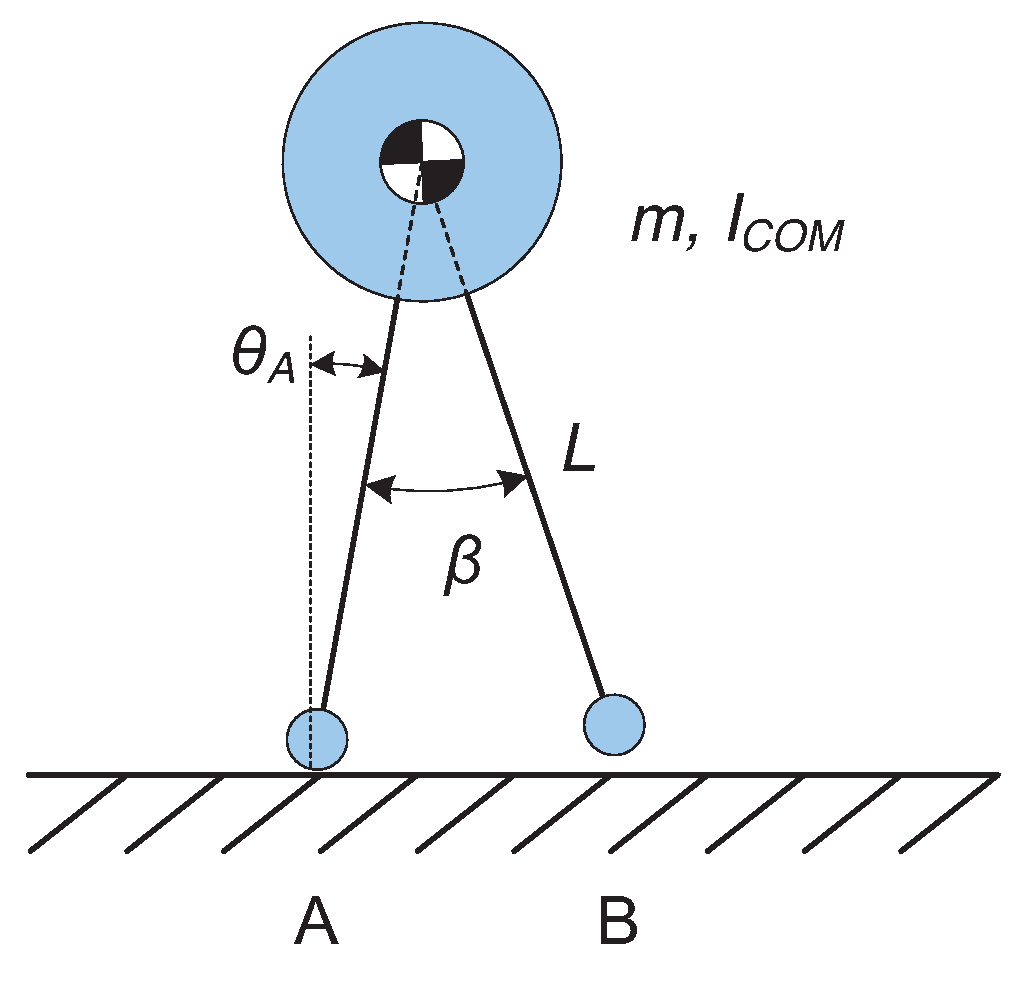
\includegraphics[scale=0.4]{fig/fpe/fig1.eps}
  	\caption{Standard compass biped model used for nonlinear analysis  and derivation of the FPE equation.}
	\label{fig:compass}
\end{figure}

Now consider this system at the moment when the swing leg comes into contact with the ground at point $B$ (the resulting behaviour is illustrated in Figure \ref{fig:prepost}). The following assumptions are made in reference to the behaviour of the system around the pre-impact and post-impact stages to simplify the model for further analysis \cite{Wight:2008vt}: 

\hrulefill

\begin{assumption}
	There is an instantaneous transfer of balance (i.e. the stance foot at point $A$ lifts up when the swing foot hits the ground at point $B$).  
\end{assumption}

\begin{assumption}
	The impact when the swing leg hits the ground at point $B$ is assumed to plastic. 
\end{assumption}

\begin{assumption}
	There is sufficient friction to prevent any slipping at the contact points. 
\end{assumption}

\begin{assumption}
	Gravity is assumed to be a non-impulsive force. 
\end{assumption}

\begin{assumption} \label{assump:betafix}
	The leg separation angle $\beta$ is fixed.
\end{assumption}

\begin{assumption} \label{assump:massless}
	The legs are massless and therefore do not significantly alter the dynamics of the system. 
\end{assumption}

\hrulefill

Note that assumption \ref{assump:betafix} implies that if both feet were to remain on the ground (i.e. double support phase), then by geometric symmetry about the normal, $\theta _A = \beta/2$. Equivalently, when leg $A$ is completely vertical, $\theta _A = 0$.

\begin{figure}[!h]
	\centering
    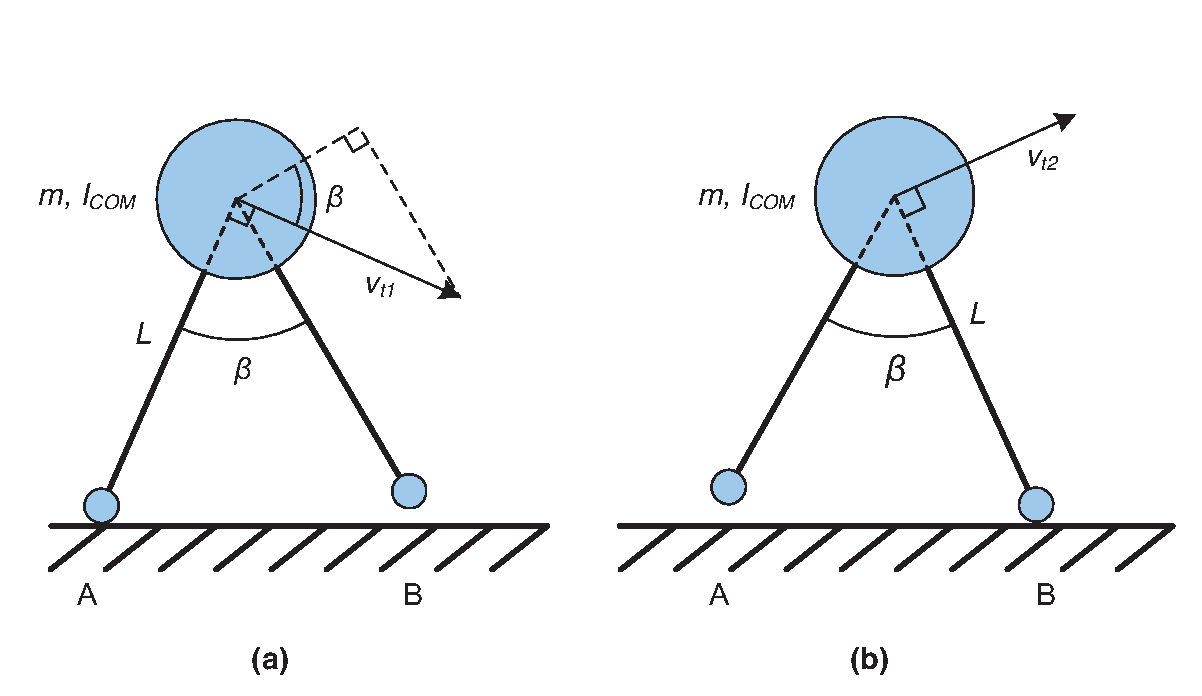
\includegraphics[scale=0.6]{fig/fpe/fig2.eps}
  	\caption{Compass biped model in the swing phase of the gait cycle in the (a) pre-impact and (b) post-impact configurations.}
	\label{fig:prepost}
\end{figure}

\subsection{Equations of Motion}

To formulate a state space representation of the biped, the equations of motion are derived as follows\footnote{Only key points of the derivation are summarized, for details on the full derivation of the FPE equation can be found in \cite{Wight:2008vt,Millard:2011vk}}. If the biped is treated as an inverted pendulum rotating about pivot point $A$ (i.e. configuration shown in Figure  \ref{fig:compass}), the equation of motion is found by applying Newton's second law:

\begin{equation}
	\begin{aligned}
		\sum {{\tau _A} = {I_A}} {{\ddot \theta }_A}
	\end{aligned}
\end{equation}

\begin{equation} \label{eq:compasseom1}
	\begin{aligned}
		{{\ddot \theta }_A} = \frac{{mgL\sin ({\theta _A})}}{{{I_{COM}} + m{L^2}}}
	\end{aligned}
\end{equation}

This equation is only valid while the inverted pendulum swings about point $A$ (i.e. pre-impact). When the swing leg comes in contact with the ground and based on the assumptions, point $B$ becomes the new pivot for inverted pendulum (post-impact). The motion of the post-impact system is now based on a different angular velocity (namely, $\dot{\theta}_B$). However, the assumptions 1-4 also relate the angular momentum of the system in the pre-impact stage (Figure \ref{fig:prepost}a) to the post-impact stage (Figure \ref{fig:prepost}b). Applying the conservation of angular momentum about point $B$, the post-impact angular velocity ($\dot{\theta}_B$) is a function of the pre-impact angular velocity ($\dot{\theta}_A$) \cite{Wight:2008vt} by the following: 

\begin{equation}
	\begin{aligned}
		{\dot \theta _B} = \frac{{({L^2}m\cos (\beta ) + {I_{COM}}){{\dot \theta }_A}}}{{{L^2}m + {I_{COM}}}}
	\end{aligned}
\end{equation}

While pivoting about point $B$, if the biped does not have enough momentum to swing all the way through then it simply rocks back until swing leg $A$ comes into contact with the ground. At this point, the equation of motion describing the system reverts back to \eqref{eq:compasseom1}. Given the geometric properties of the biped, it can be shown that the equation of motion about point $B$ is given by: 

\begin{equation} \label{eq:compasseom2}
	\begin{aligned}
		{\ddot \theta _B} = \frac{{mgL\sin ({\theta _B})}}{{{I_{COM}} + m{L^2}}} 
	\end{aligned}
\end{equation}

Together, $\theta _A$, $\theta _B$, along with its derivatives completely describe the motion of the compass biped. 

\subsection{Unified State Equations}
Assumption 5 imposes a geometric constraint which can be used to combine the variables which completely define the motion. At the instant of impact, the angles $\theta _A$ and $\theta _B$ can be expressed as: 

\begin{equation}
	\begin{aligned}
		{\theta _A} = \theta  + \frac{\beta}{2} \\
		{\theta _B} = \theta  - \frac{\beta}{2}
	\end{aligned}
\end{equation}

Where the angles $\theta _A$, $\theta _B$, $\theta$ and $\beta$ are shown on Figure \ref{fig:unified}. The single (unified) variable $\theta$ can be formed by rearranging the equations of motion described in terms of $\theta _A$ and $\theta _B$: 

\begin{subnumcases}{\ddot{\theta}=\label{eq:unifiedeom}}
	\frac{{mgL\sin (\theta  + \beta /2)}}{{{I_{COM}} + m{L^2}}} & $\theta < 0$ \\
	\frac{{mgL\sin (\theta  - \beta /2)}}{{{I_{COM}} + m{L^2}}} & $\theta > 0$ \\
	\frac{{mgL\sin (\theta  + \beta /2)}}{{{I_{COM}} + m{L^2}}} & $\theta = 0$, $\dot{\theta} > 0$ \\
	\frac{{mgL\sin (\theta  - \beta /2)}}{{{I_{COM}} + m{L^2}}} & $\theta = 0$, $\dot{\theta} < 0$ \\
	\quad \quad \quad \quad 0 & $\theta = 0$, $\dot{\theta} = 0$
\end{subnumcases}

The system defined by \eqref{eq:unifiedeom} is used to investigate stability and subsequently derive the FPE equation. For future reference, define the following function to represent conditional equation of motion corresponding to a region of the state space (defined by $\theta$ and $\dot{\theta}$): 

\begin{equation}  
	\begin{aligned}
		\ddot{\theta} \eqdef F(\theta, \dot{\theta})
	\end{aligned}
\end{equation}

\begin{figure}[!t]
	\centering
    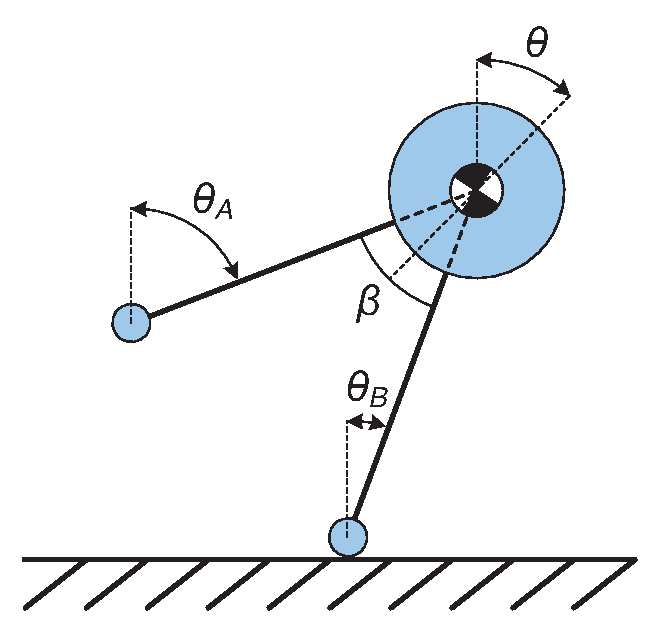
\includegraphics[scale=0.7]{fig/fpe/fig3.eps} 
  	\caption{Unified variable $\theta$ used to simplify the analysis. It is easily observed that $\theta_A = \theta  + \beta /2$ and $\theta_B = \theta  - \beta /2$}.
	\label{fig:unified}
\end{figure}

This unified variable is used to form a state space representation with the states as $\theta$ and $\dot{\theta}$: 

\begin{equation} \label{ss}
	\begin{aligned}
				\begin{gathered}
  			\dot{\Theta} = \left[ {\begin{array}{*{20}{c}}
  {\dot \theta } \\ 
  {F(\theta, \dot{\theta})} 
							   \end{array}} \right]
		\end{gathered}
	\end{aligned}
\end{equation}

\subsection{Conditions for Stability}
The notion of stability (or lack there of) is explicitly defined by \cite{Wight:2008vt} as follows: 

\hrulefill

\begin{definition} \label{def:fallen}
	The biped has fallen if $\dot{\theta} = 0$ and any other point other than the feet is in contact with the ground. 
\end{definition}

\begin{definition} \label{def:balanced}
	The biped is balanced if $\dot{\theta} = 0$ and it has not fallen. 
\end{definition}

\begin{definition} \label{def:stable}
	The biped has stable if for a given set of initial conditions and no further energy input to the system, the biped eventually comes to a rest in an upright position. Once at rest, a sufficiently small, impulsive, nonzero external disturbance to the biped should result in motion that will eventually return to the same stable, balanced position. 
\end{definition}

\hrulefill

\begin{figure*}[!t]
	\begin{equation} \label{eq:fpe}
	\begin{aligned}
		\frac{{{{\left[ {mh({v_x}\cos \phi  + {v_y}\sin \phi )\cos \phi  + {I_{COM}}{{\dot \theta }_1}{{\cos }^2}\phi } \right]}^2}}}{{m{h^2} + {I_{COM}}{{\cos }^2}\phi }} + 2mgh\cos \phi (\cos \phi  - 1) = 0
	\end{aligned}
	\end{equation}
	\\ 
	\hrulefill
\end{figure*}

The only physical configuration that can be achieved by definition \ref{def:balanced} is if the biped is double support phase. This implies that being balanced is mathematically equivalent to the system $\dot{\Theta}$ remaining at its stable equilibrium at the origin. The second part of definition \ref{def:stable} implies that stability in the physical sense is equivalent to the origin of system $\dot{\Theta}$ being asymptotically stable (since the biped should return to the same balanced position after small enough perturbations.

Thus, it is possible to determine the conditions for which the biped is stable if it it can be shown that the origin of \eqref{ss} is asymptotically stable. To this end, a Lyapunov function candidate based on the energy of the system ($U = T + V$) with an offset in potential energy is chosen to show asymptotic stability. For example, for the first equation of motion represented by \eqref{eq:unifiedeom} for $\theta < 0$: 

\begin{equation}
	\begin{aligned}
		V(\Theta) &= {\frac{1}{2}({I_{COM}} + m{L^2}){\dot \theta ^2} + mg(h - {h_{datum}})}	
		\end{aligned}
\end{equation}

Where $h =\cos (\theta+\beta/2) $ and $h_{datum} = \cos (\beta/2)$. The Lyapunov candidate is positive definite if $-\beta/2 < \theta < \beta/2$ with the following $\dot{V}(\Theta)$: 

\begin{equation}
	\begin{aligned}
			\dot{V}(\Theta) &= ({I_{COM}} + m{L^2}){\dot \theta ^2}F(\theta ,\dot \theta ) - mgL\sin (\theta  + \beta /2)\dot \theta
	\end{aligned}
\end{equation}

Analyzing the behaviour of $\dot{V}(\Theta)$ involves looking at each region of the state space specified by \eqref{eq:unifiedeom} and investigating the behaviour within the local region. In summary, $\dot{V}(\Theta) = 0$ for the cases where $\theta \not= 0$  (i.e. \ref{eq:unifiedeom}a and \ref{eq:unifiedeom}b) and is negative definite when $\theta = 0$, $\dot{\theta} \not= 0$ (i.e. \ref{eq:unifiedeom}c and \ref{eq:unifiedeom}d). Furthermore, the equilibrium point is the largest invariant set in: 
\[E = \left\{ {\Theta |\dot V(\Theta ) = 0} \right\}\]
Thus, by the Barbashin-Krasovskii-LaSalle principle it is shown that origin of $\dot{\Theta}$ is locally asymptotically stable in the sense of Lyapunov. In order to determine which initial conditions will exhibit a decaying orbit towards the origin, the exact boundaries of the local stability is obtained by analyzing the behaviour of the total system energy with different initial conditions. 

\subsection{Computing the FPE Angle} % (fold)
\label{sub:computing_the_fpe_angle}
Given that the system is asymptotically stable and the exact boundaries of the local stability are defined, it is possible to determine whether a specific location in the state space is stable in the sense of definition \ref{def:stable}. However, the goal for FPE is to determine where the foot must be placed in order to restore stability, so the knowledge of the local stability is used to reformulate the problem. 

To this end, the approach described in \cite{Wight:2008vt} introduces a parameter known as the FPE angle ($\phi$). The projection from the COM at an this angle $\phi$ to the ground surface provides the location of where the foot would need to be placed in order to restore stability to the unbalanced system. The actual solution to \eqref{eq:fpe} yields the FPE angle $\phi$, which can be obtained by using numerical techniques for solving non-linear equations. In essence, the FPE angle $\phi$ specifies the configuration system to enter/remain inside the locally stable region of $\dot{\Theta}$ if it were to step in the \textit{next} instant. By continuously tracking this angle while the biped is about to land the swing foot, the angle $\phi$ eventually converges to $\beta/2$ prior to impact.

Note that so far, the simple compass biped model used made several assumptions which are now lifted. The leg separation angle $\beta$ is no longer a fixed value throughout the whole gait cycle. Instead, by assumption \ref{assump:massless} that the legs are massless (and therefore they do not alter the dynamics of the system), the value of $\beta$ can vary while the swing leg is being brought over to the contact point for the subsequent step. The solution to the FPE equation requires only that the leg length $L$ and angle $\beta$ are fixed at the instant of impact. Simply put, the compass biped model used in the derivation thus far only represents how a real biped looks when an impact occurs. During the swing phase, an arbitrary and more realistic model of the biped looks like as shown in Figure \ref{fig:phi}, where the angle $\phi$, projection from the COM and the FPE location on the ground plane are visualized. 

\begin{figure}[h]
	\centering
    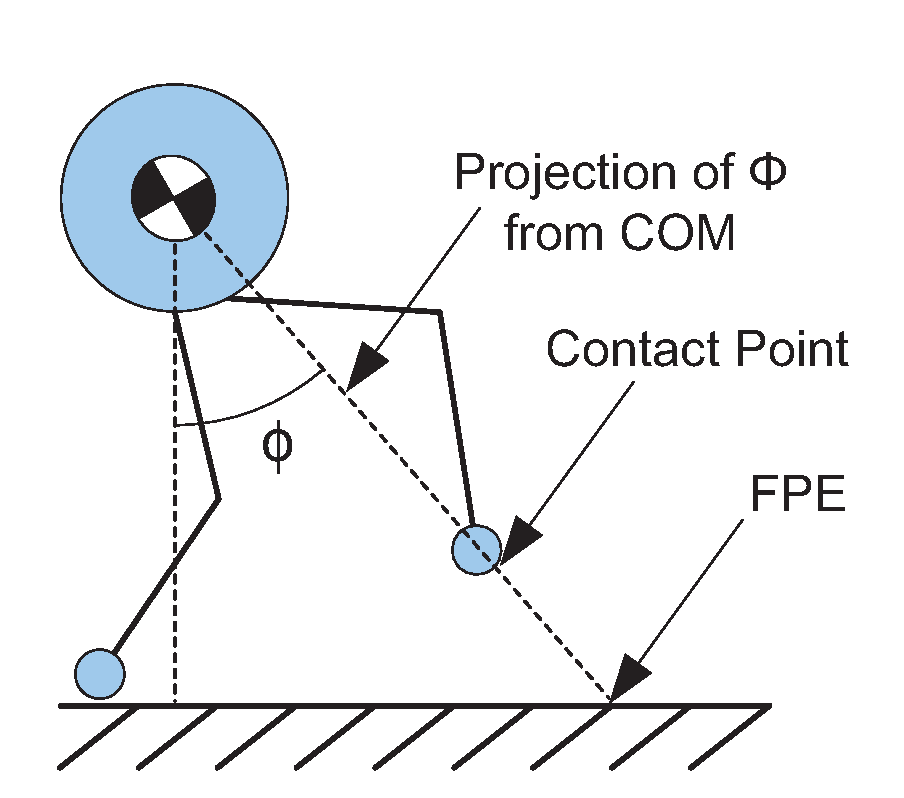
\includegraphics[scale=0.6]{fig/fpe/fig5.eps}
  	\caption{Graphical representation of the solution to the FPE equation for arbitrary robot configurations.}
	\label{fig:phi}
\end{figure}

% subsection computing_the_fpe_angle (end)

\subsection{Stability Analysis} % (fold)
\label{sub:overstepping_understepping_simulation}

In order to show that stepping on the FPE point can restore stability to an unbalanced system, the unified state space model was implemented in simulation along with a numerical solver for the nonlinear FPE equation \eqref{eq:fpe}. Three experiments were devised to analyze the behaviour of the system when the swing foot steps exactly on, behind and ahead of the FPE location obtained from the solver. These three cases are labelled perfect, under and over stepping, respectively. The simulations assume arbitrary physical parameters for $m$, $I_{COM}$, etc. The compass biped model with the single state variable is simulated to illustrate the effects of overstepping and under stepping. The leg separation angle $\beta$ is held constant and no energy is lost upon impact. 

\begin{figure}[!h]
	\begin{center}
	\subfigure{\includegraphics[scale=0.43]{fig/simulations/perfectsteppingtime.eps}}
	\subfigure{\includegraphics[scale=0.43]{fig/simulations/perfectsteppingphase.eps}}
	\end{center}
  	\caption{Time evolution and state trajectories for perfect stepping (i.e. foot lands extactly on the FPE point)}
	\label{sim:perfect}
\end{figure}

The results of the perfect stepping case shown in Figure \ref{sim:perfect} validate the efficacy of the FPE point on the ground. Starting from an unstable configuration, the simple biped model exhibits stability (i.e. rocking back and forth) due to no energy loss in the system by assumption. For a real physical biped, the energy losses experienced during impact would produce a decaying orbit towards the origin due to the asymptotic stability of the system within this local region. 

\begin{figure}[!h]
	\begin{center}
	\subfigure{\includegraphics[scale=0.43]{fig/simulations/understeppingtime.eps}}
	\subfigure{\includegraphics[scale=0.43]{fig/simulations/understeppingphase.eps}}
	\end{center}
  	\caption{Time evolution and state trajectories for under stepping (i.e. foot lands behind FPE point)}
	\label{sim:under}
\end{figure}

In the under stepping case, the swing foot lands short of the FPE location on the ground. This behaviour results in an excessive energy and momentum which causes the biped to eventually fall over. Starting from the same initial conditions presented in the perfect stepping case, the results of understepping is shown in Figure \ref{sim:under}. The time evolution and state trajectories exhibit unstable behaviour, further validating the results presented in \cite{Wight:2008ii}. 

\begin{figure}[!h]
	\begin{center}
	\subfigure{\includegraphics[scale=0.43]{fig/simulations/oversteppingtime.eps}}
	\subfigure{\includegraphics[scale=0.43]{fig/simulations/oversteppingphase.eps}}
	\end{center}
  	\caption{Time evolution and state trajectories for over stepping (i.e. foot lands in front of FPE point)}
	\label{sim:over}
\end{figure}

Lastly, the results of overstepping with the same initial conditions is presented in Figure \ref{sim:over}. As expected, if the swing foot lands ahead of the FPE location, the system enters a stable orbit where the biped rocks back and forth. As mentioned previously, the energy losses experienced during impact for a real biped would cause this closed orbit to decay and eventually reach the equilibrium due to local asymptotic stability. 

% subsection overstepping_understepping_simulation (end)

\subsection{Forming Complete Gait Cycles} % (fold)
\label{sub:gait_cycles}
Wight used the FPE concept to develop full gait cycles using simple linear control techniques and a state machine \cite{Wight:2008vt}. Gait is initiated by destabilizing the robot in the desired direction of movement (forward or backward). Once destabilized, the FPE equation is solved numerically to obtain the FPE angle $\phi$, which is used to provide the desired trajectory for the swing foot. 

\begin{figure}[!h]
	\centering
    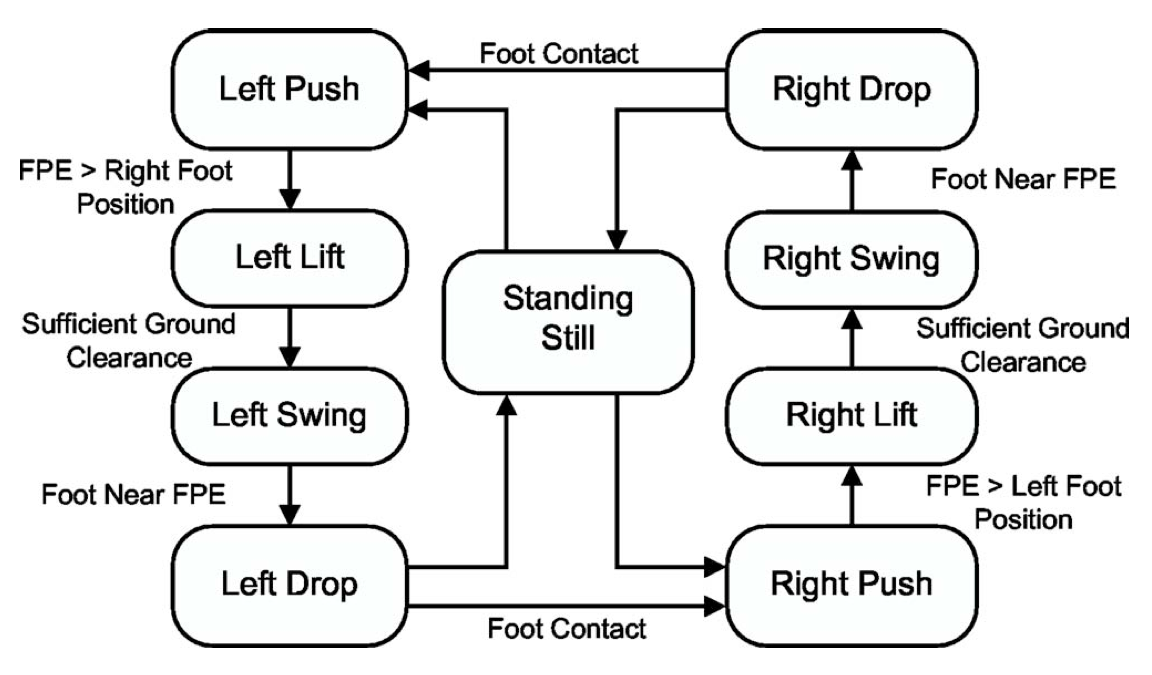
\includegraphics[scale=0.4]{fig/simulations/fpestatemachine.png}
  	\caption{A simple state machine used in conjunction with the FPE algorithm to form complete gait cycles}.
	\label{fig:statemachine}
\end{figure}

If continued forward progress is desired, the foot is commanded to precede the FPE. If no further forward progress is needed, the foot is commanded to the FPE. The desired trajectory is resolved to joint angles using inverse kinematics and implemented via joint level PD controllers. The complete state machine is shown in Figure~\ref{fig:statemachine}. Due to symmetry, the states in Figure~\ref{fig:statemachine} can be reduced to \textbf{STAND}, \textbf{PUSH}, \textbf{LIFT}, \textbf{SWING} and \textbf{DROP}. For the remainder of this paper, the sequence of state transitions from \textbf{PUSH} to \textbf{DROP} is referred to as the step cycle.
% subsection forming_complete_gait_cycles (end)


% section fpe_2D (end)
% chapter background (end) ====================================================